\chapter{Desenvolupament del Projecte}

Com part important del projecte consta del disseny d'un nou llenguatge de programació, dedicaré una secció a explicar els principis de disseny i les característiques d'aquest llenguatge, de manera que les seccions posteriors siguin més entenedores.

En una segona secció, explicaré quins són els mòduls del programa resultant i finalment entraré en detall als mòduls més importants.

\section{Disseny}

Ja s'ha dit en la introducció quins punts de disseny seguirà el llenguatge, que s'anomena Quadriga en honor a un dels esports amb més renom disputats als Jocs Olímpics Clàssics, aquí parlarem de com s'ha tractat cada punt per, posteriorment, fer un resum de la seva estructura.

\begin{description}
  \item[Open Source] \hfill \\
    El codi del projecte s'ha penjat públicament a GoogleCode sota una llicència LGPL, que permet usar-la lliurement amb la única restricció d'haver de publicar els canvis fets sobre la mateixa llibreria sota la mateixa llicència. També s'ha optat per fer servir només llibreries OpenSource com l'analitzador de sintaxi {\em JavaCC}, la llibreria gràfica {\em LWJGL} i la base de dades {\em HSQLDB}.
    
  \item[El sistema d'entitats ha de ser independent] \hfill \\
    S'ha optat per separar les {\em dades} de la funcionalitat, podent crear implementacions diferents per les mateixes dades, fent així que que fins hi tot puguem substituir totes les classes encarregades de renderitzar l'escena sense haver de tocar una línia de la definició de les entitats.
    
  \item[Ha de ser multi-plataforma de forma nativa] \hfill \\
    S'ha optat per programar sobre Java, i usar únicament llibreries escrites totalment amb Java o, en cas necessari, amb codi natiu multi-plataforma. S'intenta el màxim possible que no s'hagi de fer codi dependent de la plataforma.
    
  \item[Ha de permetre un desenvolupament ràpid un cop estiguin fets els components bàsics] \hfill \\
    S'ha intentat que la creació d'entitats i la seva interacció sigui el més senzilla possible.
    
  \item[Ha de ser fàcilment paral·lelitzable] \hfill \\
    S'han afegit expressament comportaments indefinits del programa, especialment en l'àmbit de l'ordre d'execució de certs elements, per exemple, d'ordre en que un sistema actualitza les entitats, o l'ordre en que 2 sistemes no relacionats s'actualitzen. D'aquesta manera es permet que el llenguatge mateix crei diferents fils d'execució i els balancegi de forma òptima.
\end{description}

\subsection{Definicions pròpies del llenguatge Quadriga}

Aqui explicaré les definicions bàsiques de conceptes pròpis del Sistema d'entitats Quadriga. Per a més informació consultar \cite{EntityWikiB} o \cite{Martin07}, llocs d'on he tret la inspiració bàsica per crear aquest sistema.

Esencialment es tracta de crear una API idèntica a una Base de Dades relacional on:

\begin{itemize}
  \item Les claus primàries són les "Entitats"
  \item Cada fila és un array de dades, anomenat "Component"
  \item Cada taula està associada a un "Component"
\end{itemize}

\subsubsection{Entitat}

En un nivell molt concret, una entitat és simplement un enter, o identificador, únic. A nivell més abstracte, una entitat és tot aquell objecte que apareix d'alguna manera en un joc. Pot ser des de l'avatar del jugador, als items que recull, passant per elements d'una GUI, o escenaris estàtics.

\subsubsection{Component}

Un component és un conjunt de dades que defineixen l'estat d'una entitat. Hi ha diferents tipus de components i cada un aporta diferentes dades. Cada component també du associada certa funcionalitat, però aquesta mai es troba dintre del mateix component, sinó en un sistema (tenint sempre una separació de "codi" i "dades".

\subsubsection{Sistema}

Un Sistema és un Objecte opac que s'encarrega d'una part de la funcionalitat del joc, per exemple:
\begin{description}
  \item[Physics System] s'activa cada 17ms i itera sobre totes les entitas amb física i fa un frame de simulació.
  \item[Rendering System] itera sobre totes les entitas amb representació 2D/3D i les renderitza per pantalla.
  \item[Script System] itera sobre totes les entitats que tenen un script associat i crida aquest script.
\end{description}

Un sistema sap sobre quines entitats ha d'iterar gràcies a saber quins components té associat.

\subsubsection{Thread}

Un Thread és una agrupació de sistemes que s'han d'executar en un ordre establert, seguint així unes garanties.

\subsubsection{Prototip}

Un prototip és una eina que ajuda a crear entitats. Conceptualment és semblant a una funció que inserta els components necessaris amb els parametres que toquen per crear-la. És, com el seu nom indica, el prototip de un tipus d'entitats.

\subsubsection{Main}

L'Objecte Main defineix quins threads executa l'aplicació i una funció d'inicialització de la mateixa. Quan s'executa un programa Quadriga, s'ha d'especificar el nom d'un objecte tipus Main per a executar.

\section{Estructura del Programa}

\begin{figure}
  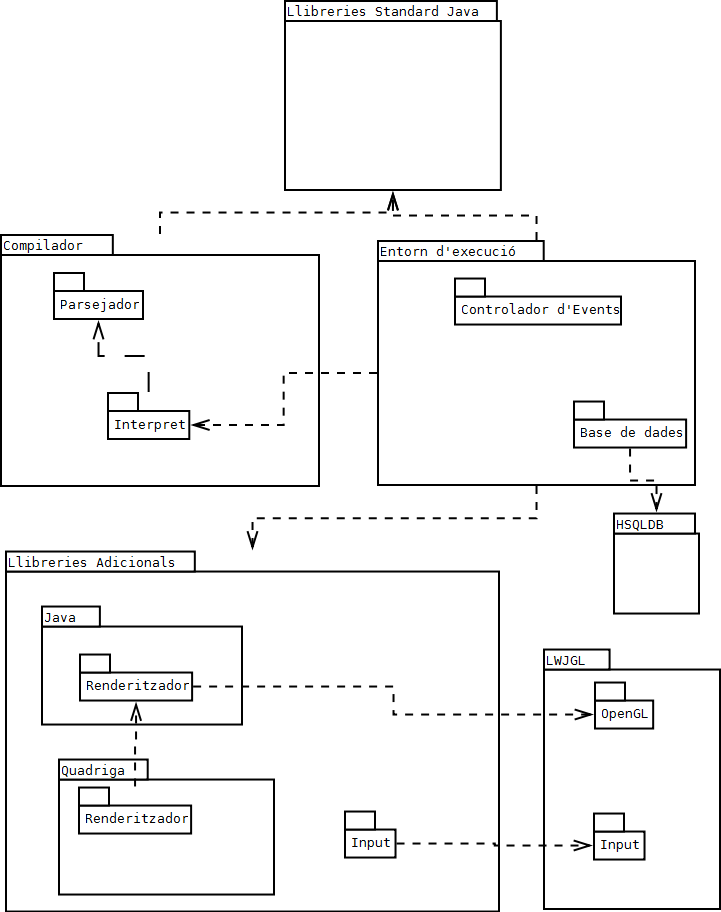
\includegraphics[width=1\linewidth]{./img/Moduls.png}
  \caption{Diagrama de mòduls \label{fig:DiagramaDeModuls}}
\end{figure}

Com es veu a la figura \ref{fig:DiagramaDeModuls}, el programa consta d'un {\em compilador}, que a partir d'un seguit de fitxers crea una estructura de dades que posteriorment és interpretada. L'execució necessita d'un {\em entorn}, que s'encarrega essencialment de les operacions pròpies de {\em quadriga} com són la creació, destrucció i cerca de components i entitats, la relació d'un component amb una entitat, l'enviament d'esdeveniments ({\em events}) entre entitats o components, etc\ldots

\section{Model de Dades}

Com ja s'ha comentat, un sistema d'entitats acava sent molt semblant a una Base de Dades relacional, on cada tipus de component equival a una taula, cada entitat a un identificador i en cada fila d'aquestes taules hi ha les dades corresponents. A més, aquesta base de dades ha de complir un seguit d'especificacions:

\begin{itemize}
  \item aaa
\end{itemize}

L'esquema Entiat-Relació resultant es mostra a la figura \ref{fig:EntitatRelacio}. I la base de dades relacional tindria la forma mostrada a la figura \ref{fig:BBDDRelacional}.

\begin{figure}
  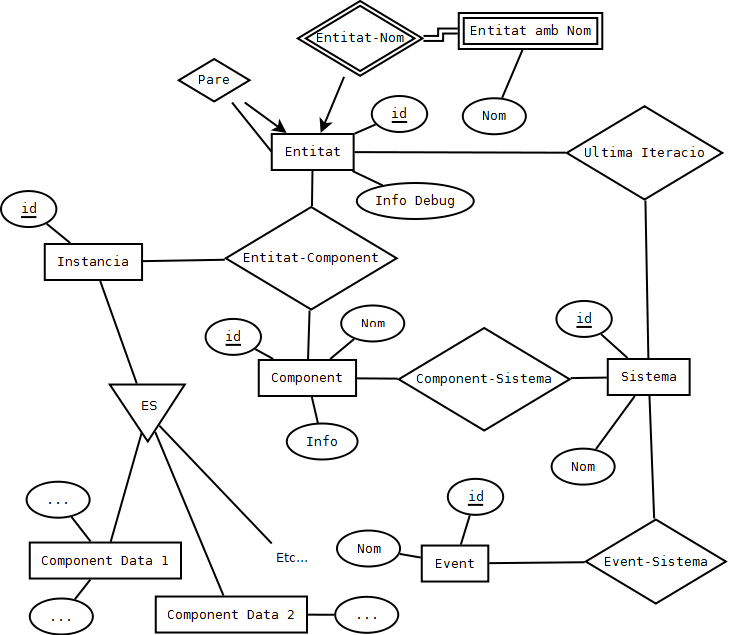
\includegraphics[width=1\linewidth]{./img/EntitatRelacio.png}
  \caption{Model Enitat-Relació \label{fig:EntitatRelacio}}
\end{figure}

\begin{figure}
  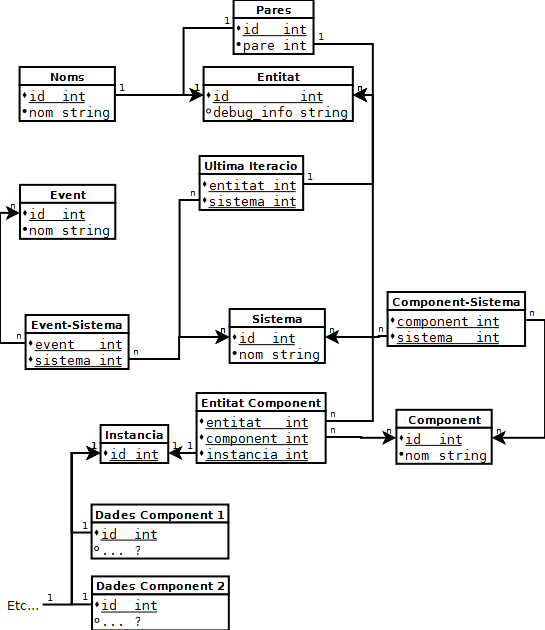
\includegraphics[width=1\linewidth]{./img/BBDDRelacional.png}
  \caption{Base de dades. \label{fig:BBDDRelacional}}
\end{figure}